% Unit 109 English translation of chapter8.tex lines 454--759.
% Source: Methods of Algebra, Volume 2, commit
% 9a5803ff77dd3257484cb177f851a73770a59dd3 (CC BY 4.0).
% stable-unit-id: o014.aljabr2.chapter8.geometric-realization
% Coverage: complete Section 8.4 on the geometric-realization functor,
% including the singular functor, the product theorem, simplicial homotopy,
% and shuffle signs; stops immediately before Section 8.5 on Dold--Kan.

% segment-id: o014.aljabr2.chapter8.geometric-realization.h001
\section{The Geometric-Realization Functor}\label{sec:geom-realization}
\hypertarget{o014.aljabr2.chapter8.geometric-realization}{ }
% segment-id: o014.aljabr2.chapter8.geometric-realization.p001
We now begin to build a geometric picture of the simplicial sets introduced
in \S\ref{sec:simplicial-set}. We start with the standard $n$-simplex, where
$n\in\Z_{\geq0}$. Write the standard ordered basis of $\R^{n+1}$ as
$e_0,\ldots,e_n$. Define
% segment-id: o014.aljabr2.chapter8.geometric-realization.q001
\[
|\Delta^n| := \left\{ (x_0, \ldots, x_n) \in (\R_{\geq 0})^{n+1} : \sum_{i=0}^n x_i = 1 \right\} \quad
\begin{tikzpicture}[baseline=(O)]
	\coordinate (O) at (0, 0);
	\draw[-Latex] (0, 0) -- (-0.7, -0.7) node[left] {$e_0$};
	\draw[-Latex] (0, 0) -- (1, 0) node[right] {$e_1$};
	\draw[-Latex] (0, 0) -- (0, 1) node [above] {$e_2$};
	\fill[color=gray, opacity=0.4] (-0.4, -0.4) -- (0.75, 0) -- (0, 0.75) --cycle;
	\node at (1, -0.7) {(the special case $n=2$)};
\end{tikzpicture}
\]
Its vertices are labeled $0,\ldots,n$ by $i\leftrightarrow e_i$. Its
interior is given the standard orientation for which
$e_1-e_0,\ldots,e_n-e_{n-1}$ is a positively oriented basis at every point.

% segment-id: o014.aljabr2.chapter8.geometric-realization.p002
Every monotone map $f:[m]\to[n]$ induces a map
% segment-id: o014.aljabr2.chapter8.geometric-realization.q002
\[\begin{tikzcd}[row sep=tiny]
	{|f|}: {|\Delta^m|} \arrow[r] & {|\Delta^n|} \\
	\sum_{i=0}^m y_i e_i \arrow[mapsto, r] & \sum_{i=0}^m y_i e_{f(i)}.
\end{tikzcd}\]
If $f$ is not surjective, the image of $|f|$ lies in the boundary. The
embedding $|\mathrm{d}^i|:|\Delta^{n-1}|\to|\Delta^n|$ may be used to
compare the orientation on the interior of $|\Delta^{n-1}|$ with the
orientation induced on the boundary by $|\Delta^n|$. A standard determinant
calculation shows that they differ by a factor of $(-1)^i$. The following
figure illustrates the case $n=2$.
% segment-id: o014.aljabr2.chapter8.geometric-realization.g001
\begin{center}
	\begin{tikzpicture}
		\coordinate (A) at (0, 0);
		\coordinate (B) at (2, 0);
		\coordinate (C) at (1, 1.2);
		\fill[color=gray, opacity=0.25] (A) -- (B) -- (C) --cycle;
		\draw[ultra thick] (A) -- (B) -- (C) -- (A);
		\node[shape=circle, inner sep=0.3em, fill=white, draw] at (A) {$0$};
		\node[shape=circle, inner sep=0.3em, fill=white, draw] at (B) {$1$};
		\node[shape=circle, inner sep=0.3em, fill=white, draw] at (C) {$2$};

		\draw ($(B) + (0.8, 0.8)$) node[shape=rectangle, inner sep=0.3em, draw, below] {$0$} -- ($(C) + (0.8, 0.8)$) node[shape=rectangle, inner sep=0.3em, draw, above] {$1$};
		\draw[-Latex] ($(C)!0.5!(B) + (0.7, 0.7)$) to[edge label={$\mathrm{d}^0$}, swap] ($(C)!0.5!(B) + (0.2, 0.2)$);

		\draw ($(A) + (-0.8, 0.8)$) node[shape=rectangle, inner sep=0.3em, draw, below left] {$0$} -- ($(C) + (-0.8, 0.8)$) node[shape=rectangle, inner sep=0.3em, draw, above right] {$1$};
		\draw[-Latex] ($(A)!0.5!(C) + (-0.7, 0.7)$) to[edge label={$\mathrm{d}^1$}] ($(A)!0.5!(C) + (-0.2, 0.2)$);

		\draw ($(A) + (0, -1.2)$) node[shape=rectangle, inner sep=0.3em, draw, left] {$0$} -- ($(B) + (0, -1.2)$) node[shape=rectangle, inner sep=0.3em, draw, right] {$1$};
		\draw[-Latex] ($(A)!0.5!(B) + (0, -1)$) to[edge label={$\mathrm{d}^2$}] ($(A)!0.5!(B) + (0, -0.3)$);

		\node at (5, 2) {Orientation:};
		\node (U) at (6.5, 2) {$0$};
		\node (V) at (8.5, 2) {$1$};
		\draw[->] (U) -- (V);
		\node (X) at (6.5, 0) {$0$};
		\node (Y) at (8.5, 0) {$1$};
		\node (Z) at (7.5, 1.2) {$2$};
		\draw[->] (X) -- (Y);
		\draw[->] (Y) -- (Z);
		\draw[->] (Z) -- (X);
	\end{tikzpicture}
\end{center}

% segment-id: o014.aljabr2.chapter8.geometric-realization.p003
Summarizing the discussion above, we obtain a functor
% segment-id: o014.aljabr2.chapter8.geometric-realization.q003
\begin{equation*}
	|\cdot|: \simpDelta \to \cate{Top} \quad
	\left\{\begin{array}{ll}
		\text{objects} & [n] \mapsto |\Delta^n| \\
		\text{morphisms} & f \mapsto |f| .
	\end{array}\right.
\end{equation*}
We wish to extend it to a functor $\cate{sSet}\to\cate{Top}$. Recall that
$\cate{Top}$ is cocomplete.

% segment-id: o014.aljabr2.chapter8.geometric-realization.d001
\begin{definition}[Geometric-realization functor]
	\index{geometric realization}
	\index[sym1]{X-realization@$\lvert X\rvert$}
	The functor $|\cdot|:\cate{sSet}\to\cate{Top}$ is defined as follows. If
	$X$ is a simplicial set, then
% segment-id: o014.aljabr2.chapter8.geometric-realization.q004
	\[ |X| := \varinjlim_{n, x} |\Delta^n|, \]
	where $n\in\Z_{\geq0}$ and $x\in X_n$, or equivalently, where $x$ is a
	morphism $\Delta^n\to X$. Such pairs $(n,x)$ form a category. A morphism
	from $(n,x)$ to $(m,y)$ is precisely an
	$f\in\Hom_{\simpDelta}([n],[m])$ for which the diagram
% segment-id: o014.aljabr2.chapter8.geometric-realization.q005
	\[\begin{tikzcd}[column sep=small]
		\Delta^n \arrow[rr, "f"] \arrow[rd, "x"'] & & \Delta^m \arrow[ld, "y"] \\
		& X &
	\end{tikzcd}\]
	commutes; equivalently, $f^*:X_m\to X_n$ must satisfy $f^*(y)=x$.
\end{definition}

% segment-id: o014.aljabr2.chapter8.geometric-realization.p004
For fixed $m\geq0$, the category of data
$(n,x:\Delta^n\to\Delta^m)$ has the terminal object
$(m,\identity_{\Delta^m})$. Therefore the geometric realization of
$\Delta^m$ is canonically identified with the previously defined
$|\Delta^m|$. Thus the notation is consistent.

% segment-id: o014.aljabr2.chapter8.geometric-realization.r001
\begin{remark}\label{rem:simplicial-density}
	For every simplicial set $X$, there is a canonical isomorphism
	$\varinjlim_{n,x}\Delta^n\rightiso X$. This follows directly by applying
	the Density Theorem~\ref{prop:Yoneda-density} to the category
	$\cate{sSet}=\simpDelta^{\wedge}$; the reader is invited to check it.
\end{remark}

% segment-id: o014.aljabr2.chapter8.geometric-realization.r002
\begin{remark}
	By Theorem~\ref{prop:Kan-limit}, geometric realization is the left Kan
	extension of the functor $|\cdot|:\simpDelta\to\cate{Top}$ along
	$\simpDelta\to\cate{sSet}$; see Definition~\ref{def:Kan-extension}.
	Thus the construction is entirely natural.
\end{remark}

% segment-id: o014.aljabr2.chapter8.geometric-realization.p005
By the construction above, for each $n\in\Z_{\geq0}$ and $x\in X_n$, the
universal property of $\varinjlim$ gives a canonical map
$i_{n,x}:|\Delta^n|\to|X|$, compatible as $(n,x)$ varies. Taking
$\varinjlim$ in $\cate{Top}$ is simply the operation of gluing topological
spaces. More concretely, the geometric realization can be written as the
quotient space
% segment-id: o014.aljabr2.chapter8.geometric-realization.q006
\begin{equation}\label{eqn:geom-realization-quotient}
	|X| = \dfrac{\displaystyle\bigsqcup_{n \geq 0} X_n \times |\Delta^n| }{(f^*(y), t) \sim (y, |f|(t)) }, \quad
	\begin{tikzcd}[column sep=tiny]
		(f^*(y), t) \arrow[phantom, r, "\in" description] & X_n \arrow[phantom, r, "\times" description] & {|\Delta^n|} \arrow[d, "{|f|}"] & {[n]} \arrow[d, "f"] \\
		(y, {|f|}(t)) \arrow[phantom, r, "\in" description] & X_m \arrow[phantom, r, "\times" description] \arrow[u, "{f^*}"] & {|\Delta^m|} & {[m]}.
	\end{tikzcd}
\end{equation}

% segment-id: o014.aljabr2.chapter8.geometric-realization.p006
In keeping with the geometric intuition, a simplicial set $X$ may be viewed
as a model of a space. The sets $X_0,X_1,\ldots$ are the collections of
building blocks of the model: each element of $X_n$ corresponds to, and
labels, one copy of $|\Delta^n|$. The various maps $f^*:X_m\to X_n$ serve as
assembly instructions that determine how these copies of $|\Delta^n|$ are
glued together.

% segment-id: o014.aljabr2.chapter8.geometric-realization.p007
Since the morphisms in $\simpDelta$ have already been described explicitly,
the equivalence relation in \eqref{eqn:geom-realization-quotient} can be
generated by two special kinds of $f$.
% segment-id: o014.aljabr2.chapter8.geometric-realization.l001
\begin{itemize}
% segment-id: o014.aljabr2.chapter8.geometric-realization.i001
	\item Take $\mathrm{d}^i:[n-1]\hookrightarrow[n]$. Then
	$|\mathrm{d}^i|$ embeds
	$\{d_i(x)\}\times|\Delta^{n-1}|$ into
	$\{x\}\times|\Delta^n|$. Thus the face map
	$d_i:X_n\to X_{n-1}$ labels the $i$th face of the $n$-dimensional
	component corresponding to $x$ by $d_i(x)$, and the gluing is then
	performed according to these labels.

% segment-id: o014.aljabr2.chapter8.geometric-realization.i002
	\item Take $\mathrm{s}^j:[n+1]\twoheadrightarrow[n]$. Then
	$|\mathrm{s}^j|$ ``collapses''
	$\{s_j(x)\}\times|\Delta^{n+1}|$ onto
	$\{x\}\times|\Delta^n|$. Thus the degeneracy map
	$s_j:X_n\to X_{n+1}$ determines how an $n$-dimensional component
	corresponding to $x$ gives rise to a ``degenerate'' $(n+1)$-dimensional
	component, labeled $s_j(x)$, which is collapsed onto its $j$th face during
	the gluing process.
\end{itemize}
% segment-id: o014.aljabr2.chapter8.geometric-realization.p008
Consequently, degenerate $n$-simplices (Definition~\ref{def:simplex}) may be
omitted from the gluing process, but the degeneracy data still cannot be
ignored. For example, a face map $d_i:X_n\to X_{n-1}$ may well map a
nondegenerate simplex to a degenerate simplex.

% segment-id: o014.aljabr2.chapter8.geometric-realization.eg001
\begin{example}
	As an illustration, $\partial\Delta^n$ in Example~\ref{eg:boundary-horn}
	realizes the boundary of the standard $n$-simplex in the intuitive sense,
	while the horn $\Lambda^n_k$ is obtained by removing from
	$\partial\Delta^n$ the face opposite its $k$th vertex. Here is one
	illustration:
% segment-id: o014.aljabr2.chapter8.geometric-realization.g002
	\begin{center}\begin{tikzpicture}
		\coordinate (A) at (0, 0);
		\coordinate (B) at (2, 0);
		\coordinate (C) at (1, 0.8);
		\coordinate (O) at (1, -1.5);

		\filldraw[thick, shading=radial, inner color=black!90, outer color=white] (A) node[left] {$1$} -- (C) node[above] {$3$} -- (B) node[right] {$2$} --($(O)!0.15!(C)$) --cycle;
		\draw (C) -- (O) node[below] {$0$};
		\filldraw[fill=white, thick] (A) -- (B) -- (O) --cycle;

		\node at ($(A) + (-1.5, -0.2)$) {$|\Lambda^3_0| =$};
	\end{tikzpicture}\end{center}
\end{example}

% segment-id: o014.aljabr2.chapter8.geometric-realization.eg002
\begin{example}\label{eg:cone-realization}
	\index{simplicial set!cone}
	For every topological space $\mathcal{X}$, define the cone over it,
	$\Cone_{\mathrm{top}}(\mathcal{X})$, to be the space obtained by
	contracting the closed subset $\mathcal{X}\times\{0\}$ of
	$\mathcal{X}\times[0,1]$ to a single point. Visually,
% segment-id: o014.aljabr2.chapter8.geometric-realization.g003
	\[\Cone_{\mathrm{top}}(\mathcal{X}) = \; 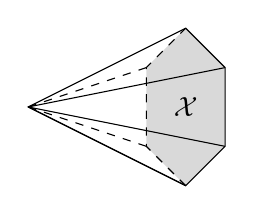
\begin{tikzpicture}[baseline=(P)]
		\coordinate (A) at (0, 1);
		\coordinate (B) at (0.5, 0.5);
		\coordinate (C) at (0.5, -0.5);
		\coordinate (D) at (0, -1);
		\coordinate (E) at (-0.5, -0.5);
		\coordinate (F) at (-0.5, 0.5);
		\coordinate (O) at (-2, 0);
		\coordinate (P) at (0, -0.1);	% For the baseline

		\fill[gray!50, opacity=0.6] (A) -- (B) -- (C) -- (D) -- (E) -- (F) --cycle;
		\draw (O) -- (A) -- (B) -- (C) -- (D) --cycle;
		\draw (O) -- (B);
		\draw (O) -- (C);
		\draw (O) -- (D);
		\draw[dashed] (D) -- (E) -- (F) -- (A);
		\draw[dashed] (O) -- (E);
		\draw[dashed] (O) -- (F);
		\node at (0, 0) {$\mathcal{X}$};
	\end{tikzpicture}\]
	As a simple exercise, check that
	$|X^{\lhd}|\simeq\Cone_{\mathrm{top}}(|X|)\simeq|X^{\rhd}|$. This shows
	that the cones in Definition~\ref{def:cone-simplicial} are aptly named;
	the only difference between the left and right cones is their orientation.
\end{example}

% segment-id: o014.aljabr2.chapter8.geometric-realization.p009
By presenting a triangulation of a space as a simplicial set, one can extract
many important topological properties. This approach is aptly called
``combinatorial topology''. Further discussion and examples may be found in
\cite[Chapter VI]{You}.

% segment-id: o014.aljabr2.chapter8.geometric-realization.d002
\begin{definition}[Singular-set functor]
	\index[sym1]{Sing@$\mathrm{Sing}$}
	\index{singular set}
	For every topological space $E$, define the simplicial set
	$\mathrm{Sing}(E)$ by
% segment-id: o014.aljabr2.chapter8.geometric-realization.q007
	\[ \mathrm{Sing}(E)_n := \Hom_{\cate{Top}}(|\Delta^n|, E), \quad n \in \Z_{\geq 0}, \]
	where $d_i:\mathrm{Sing}(E)_n\to\mathrm{Sing}(E)_{n-1}$
	(respectively, $s_j:\mathrm{Sing}(E)_n\to\mathrm{Sing}(E)_{n+1}$) is
	given by pullback along
	$|\mathrm{d}^i|:|\Delta^{n-1}|\to|\Delta^n|$ (respectively,
	$|\mathrm{s}^j|:|\Delta^{n+1}|\to|\Delta^n|$). This is called the
	\emph{(simplicial) singular set} associated with $E$. The construction
	gives a functor
% segment-id: o014.aljabr2.chapter8.geometric-realization.q008
	\[ \mathrm{Sing}: \cate{Top} \to \cate{sSet}. \]
\end{definition}

% segment-id: o014.aljabr2.chapter8.geometric-realization.th001
\begin{theorem}\label{prop:geom-Sing-adjunction}
	The geometric-realization functor is left adjoint to the singular-set
	functor. In other words, there is a natural bijection
% segment-id: o014.aljabr2.chapter8.geometric-realization.q009
	\[\begin{tikzcd}[row sep=tiny]
		\Hom_{\cate{Top}}(|X|, E) \arrow[leftrightarrow, r, "1:1"] & \Hom_{\cate{sSet}}(X, \mathrm{Sing}(E)) \\
		\varphi \arrow[mapsto, r] & {\left[ X_n \xrightarrow{x \mapsto \varphi \circ i_{n, x}} \Hom_{\cate{Top}}(|\Delta^n|, E) \right]} \\
		\displaystyle\varinjlim_{(n, x)} \left( |\Delta^n| \xrightarrow{\psi_n(x)} E \right) & \psi = {\left[ \psi_n: X_n \to \Hom_{\cate{Top}}(|\Delta^n|, E) \right]}_{n \geq 0} , \arrow[mapsto, l]
	\end{tikzcd}\]
	where $X\in\Obj(\cate{sSet})$ and $E\in\Obj(\cate{Top})$.
\end{theorem}
% segment-id: o014.aljabr2.chapter8.geometric-realization.pf001
\begin{proof}
	Recall that $|X|=\varinjlim_{n,x}|\Delta^n|$. There are canonical
	isomorphisms
% segment-id: o014.aljabr2.chapter8.geometric-realization.q010
	\begin{align*}
		\Hom_{\cate{Top}}\left( \varinjlim_{n, x} |\Delta^n| , E \right) & \rightiso \varprojlim_{n, x} \Hom_{\cate{Top}}(|\Delta^n|, E) = \varprojlim_{n, x} \mathrm{Sing}(E)_n \\
		& \rightiso \varprojlim_{n, x} \Hom_{\cate{sSet}}\left( \Delta^n, \mathrm{Sing}(E) \right) \\
		\varphi & \mapsto \left( \psi_n(x) := \varphi \circ i_{n, x} \right)_{n, x}.
	\end{align*}

	Every family of morphisms $(\psi_n(x))_{n,x}$ determined by a morphism
	$\psi:X\to\mathrm{Sing}(E)$ satisfies the compatibility conditions, and
	thus is an element of the inverse limit on the right-hand side above. To
	complete the proof, it remains to show that giving a morphism $\psi$ is
	equivalent to giving a compatible family of morphisms; this is exactly what
	Remark~\ref{rem:simplicial-density} guarantees.
\end{proof}

% segment-id: o014.aljabr2.chapter8.geometric-realization.r003
\begin{remark}
	For homotopy theory, the category $\cate{CGHaus}$ mentioned in
	\S\ref{sec:closed-monoidal} may be more convenient than $\cate{Top}$.
	Since the inclusion functor $\cate{CGHaus}\to\cate{Top}$ has a right
	adjoint $k$, it preserves $\varinjlim$. Moreover, $|\Delta^n|$ is a
	compactly generated Hausdorff space. Consequently, the gluing
	(respectively, the formation of $\Hom$) in geometric realization
	(respectively, the singular set) may be carried out within
	$\cate{CGHaus}$\footnote{It must be explained that the $\varinjlim$ in
	question does indeed exist in $\cate{CGHaus}$. This is a topological issue;
	see \cite[III.1.8, III.2.1]{GZ67}.}. Thus the adjoint pair of
	Theorem~\ref{prop:geom-Sing-adjunction} factors into two adjunctions, written
	with the same notation as
% segment-id: o014.aljabr2.chapter8.geometric-realization.q011
	\[\begin{tikzcd}
		\cate{sSet} \arrow[shift left, r, "{|\cdot|}"] & \cate{CGHaus} \arrow[shift left, r, "\text{inclusion functor}"] \arrow[shift left, l, "\mathrm{Sing}"] & \cate{Top} \arrow[shift left, l, "k"] .
	\end{tikzcd}\]
\end{remark}
% segment-id: o014.aljabr2.chapter8.geometric-realization.p010
For any two simplicial sets $X$ and $Y$, their product is defined degreewise:
% segment-id: o014.aljabr2.chapter8.geometric-realization.q012
\begin{gather*}
	(X \times Y)_n = X_n \times Y_n, \\
	d_i(x, y) = (d_i(x), d_i(y)), \\
	s_j(x, y) = (s_j(x), s_j(y)).
\end{gather*}
This is both the categorical product in
$\cate{sSet}=\cate{Set}^{\simpDelta^{\opp}}$ and the construction of
Definition~\ref{def:monoidal-sObj} applied to the monoidal category
$(\cate{Set},\times)$. Although both definitions arise from category theory,
the following fundamental result shows that they also have geometric meaning.

% segment-id: o014.aljabr2.chapter8.geometric-realization.th002
\begin{theorem}\label{prop:realization-product}
	For simplicial sets $X$ and $Y$, there is a canonical isomorphism in
	$\cate{CGHaus}$
% segment-id: o014.aljabr2.chapter8.geometric-realization.q013
	\[ |X \times Y| \simeq |X| \times |Y|. \]
	More generally, the $\cate{CGHaus}$-valued version of $|\cdot|$ preserves
	finite limits. If either $X$ or $Y$ has only finitely many nondegenerate
	simplices, then $|X\times Y|\simeq|X|\times|Y|$ also holds in
	$\cate{Top}$.
\end{theorem}

% segment-id: o014.aljabr2.chapter8.geometric-realization.p011
The proof in the general case is rather involved; see
\cite[Chapter III]{GZ67} or \cite{Dri03}. The isomorphism does not hold in
general for the $\cate{Top}$-valued version of geometric realization. Notice
also that the condition stated in the theorem for the $\cate{Top}$-valued
version is not optimal.

% segment-id: o014.aljabr2.chapter8.geometric-realization.c001
\begin{corollary}
	Write $\cate{Grp}$ for the category of groups. If a simplicial set $X$ can
	be promoted to an object of $\cate{sGrp}$, then $|X|$ naturally has the
	structure of a topological group. Analogous results hold for other
	algebraic structures.
\end{corollary}

% segment-id: o014.aljabr2.chapter8.geometric-realization.p012
In view of Theorem~\ref{prop:realization-product}, it is natural to define a
homotopy from $g$ to $f$, for morphisms $f,g:X\rightrightarrows Y$ in
$\cate{sSet}$, as a morphism $H:X\times\Delta^1\to Y$ making the following
diagram commute:
% segment-id: o014.aljabr2.chapter8.geometric-realization.q014
\begin{equation}\label{eqn:simplicial-homotopy-prep}
	\begin{tikzcd}
		X \times \Delta^0 \arrow[d, "{\identity_X \times \mathrm{d}^0}"'] \arrow[r, "\sim"] & X \arrow[d, "f"] \\
		X \times \Delta^1 \arrow[r, "H" description] & Y \\
		X \times \Delta^0 \arrow[u, "{\identity_X \times \mathrm{d}^1}"] \arrow[r, "\sim"'] & X \arrow[u, "g"']
	\end{tikzcd}
\end{equation}

% segment-id: o014.aljabr2.chapter8.geometric-realization.p013
As a special case, the composite
$X\times\Delta^1\xrightarrow{\text{projection}}X\xrightarrow{f}Y$ gives a
constant homotopy from $f$ to itself. Homotopy as defined here is not,
however, an equivalence relation: a simple example already shows that it need
not be symmetric. In homotopy theory one usually imposes an additional
condition on $Y$, for example that it be a Kan complex. The homotopy relation
then has the expected properties, allowing homotopy groups, weak
equivalences, and related notions to be studied combinatorially.

% segment-id: o014.aljabr2.chapter8.geometric-realization.p014
Although this book does not prove Theorem~\ref{prop:realization-product}, it
is useful to say a little more about the simple special case
$X=\Delta^p$ and $Y=\Delta^q$. For example, how can the nondegenerate
simplices of $\Delta^p\times\Delta^q$ be classified? The answer not only
helps explain the geometric realization of a product; the related
construction will also be needed later.

% segment-id: o014.aljabr2.chapter8.geometric-realization.p015
First, the product of two partially ordered sets $S_1$ and $S_2$ becomes a
partially ordered set under
$(a_1,a_2)\leq(b_1,b_2)$ if and only if $a_1\leq b_1$ and $a_2\leq b_2$.
This is also the product of the corresponding categories.

% segment-id: o014.aljabr2.chapter8.geometric-realization.d003
\begin{definition}\label{def:pq-shuffle}
	\index{shuffle!$(p,q)$}
	Let $p,q\in\Z_{\geq0}$. A \emph{$(p,q)$-shuffle} is an injective monotone
	map $\sigma:[p+q]\to[p]\times[q]$.
\end{definition}

% segment-id: o014.aljabr2.chapter8.geometric-realization.p016
For every $n\in\Z_{\geq0}$, specifying a monotone map
$\sigma:[n]\to[p]\times[q]$ is equivalent to specifying a pair of monotone
maps $\sigma_-:[n]\to[p]$ and $\sigma_+:[n]\to[q]$. It is also equivalent
to specifying an $n$-simplex of $\Delta^p\times\Delta^q$. The condition that
$\sigma$ be injective says precisely that the path
$i\mapsto(\sigma_-(i),\sigma_+(i))$ never remains stationary, for
$i=0,\ldots,n$. When $n=p+q$, the situation may be pictured as follows:
% segment-id: o014.aljabr2.chapter8.geometric-realization.q015
\begin{equation}\label{eqn:pq-shuffle-diag}
	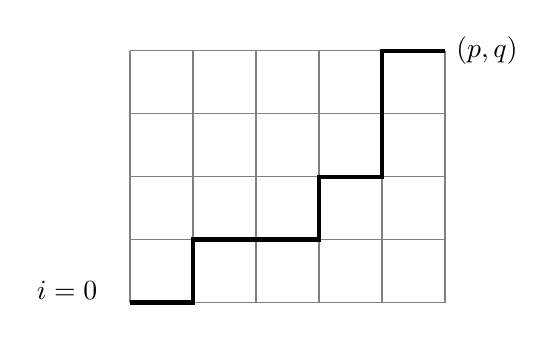
\begin{tikzpicture}[scale=0.8, baseline=(O)]
		\draw[thin, gray] (0, 0) grid (5, 4);
		\node at (-1, 0.2) {$i=0$};
		\draw[ultra thick] (0, 0) -- (1, 0) -- (1, 1) -- (2, 1) -- (3, 1) -- (3, 2) -- (4, 2) -- (4, 3) -- (4, 4) -- (5, 4) node[right] {$(p, q)$};
		\coordinate (O) at (0, 2);
	\end{tikzpicture}
	\quad
	\text{exactly $p+q$ steps.}
\end{equation}
Thus, for a $(p,q)$-shuffle $\sigma$, define
% segment-id: o014.aljabr2.chapter8.geometric-realization.q016
\begin{align*}
	I_\pm & := \left\{ 1 \leq i \leq p+q : \sigma_\pm(i-1) < \sigma_\pm(i) \right\} \\
	& = \left\{ 1 \leq i \leq p+q : \sigma_\pm(i-1) = \sigma_\pm(i) - 1 \right\} \\
	& = \left\{ 1 \leq i \leq p+q: \sigma_\mp(i-1) = \sigma_\mp(i) \right\},
\end{align*}
so that $I_+\sqcup I_-=\{1,\ldots,p+q\}$. The subsets $I_+$ and $I_-$
correspond, respectively, to the upward and rightward portions of the path in
\eqref{eqn:pq-shuffle-diag}. Thus a $(p,q)$-shuffle may also be viewed as an
ordering of $p$ symbols $\rightarrow$ and $q$ symbols $\uparrow$; there are
$\binom{p+q}{p}$ such orderings. These observations also show that
$\sigma_+$ and $\sigma_-$ are surjective monotone maps for every
$(p,q)$-shuffle.

% segment-id: o014.aljabr2.chapter8.geometric-realization.pr001
\begin{proposition}
	Let $p,q\in\Z_{\geq0}$. Consider an $n$-simplex of
	$\Delta^p\times\Delta^q$, that is, a monotone map
	$\sigma:[n]\to[p]\times[q]$. Set $(p_i,q_i):=\sigma(i)$ and
	$(p',q'):=(p_n-p_0,q_n-q_0)$. Then $\sigma$ is nondegenerate if and only if
	the following conditions hold:
	\begin{itemize}
		\item $p'+q'=n$;
		\item $\sigma$ factors as a $(p',q')$-shuffle
		$\sigma':[n]\to[p']\times[q']$ followed by a monotone injection
		$[p']\times[q']\hookrightarrow[p]\times[q]$ of the form $f\times g$.
	\end{itemize}
\end{proposition}
% segment-id: o014.aljabr2.chapter8.geometric-realization.pf002
\begin{proof}
	Identify $\sigma$ with the pair of monotone maps
	$(\sigma_-,\sigma_+)$. Consider the path $i\mapsto(p_i,q_i)$ as in
	\eqref{eqn:pq-shuffle-diag}. The condition that $\sigma$ be nondegenerate
	is equivalent to the condition that this path never remains stationary.
	The rest is clear.
\end{proof}

% segment-id: o014.aljabr2.chapter8.geometric-realization.p017
Using this description of the nondegenerate simplices, the reader may
visualize the isomorphism
$|\Delta^p\times\Delta^q|\simeq|\Delta^p|\times|\Delta^q|$ in the cases
$(p,q)=(1,1)$ and $(2,1)$. For example, the following figure shows the
triangulation of $|\Delta^2|\times|\Delta^1|$ into three tetrahedra,
corresponding to the $3=\binom{3}{2}$ $(2,1)$-shuffles.

% segment-id: o014.aljabr2.chapter8.geometric-realization.g004
\begin{center}\begin{tikzpicture}[yscale=0.8]
	\coordinate (A) at (0, 0);
	\coordinate (B) at (2.2, 0.5);
	\coordinate (C) at (0.8, -0.5);
	\coordinate (P) at ($(A) + (0, -3)$);
	\coordinate (Q) at ($(B) + (0, -3)$);
	\coordinate (R) at ($(C) + (0, -3)$);

	\draw ($(A) + (-5, -0.3)$) -- ($(B) + (-5, -0.3)$) -- ($(Q) + (-5, -0.3)$) -- ($(R) + (-5, -0.3)$) -- ($(P) + (-5, -0.3)$) --cycle;
	\draw ($(A) + (-5, -0.3)$) -- ($(C) + (-5, -0.3)$) -- ($(B) + (-5, -0.3)$);
	\draw ($(C) + (-5, -0.3)$) -- ($(R) + (-5, -0.3)$);
	\draw[dashed] ($(P) + (-5, -0.3)$) -- ($(Q) + (-5, -0.3)$);

	\draw[-Latex] ($(B)!0.5!(Q) + (-4.5, -0.5)$) -- ($(B)!0.5!(Q) + (-3, -0.5)$);

	\draw (A) -- (B) -- (C) --cycle;
	\draw (A) -- (P) -- (C);
	\draw (P) -- (B);

	\draw[fill=white] ($(P) + (0.2, -1.2)$) -- ($(B) + (0.2, -1.2)$) -- ($(R) + (0.2, -1.2)$) --cycle;
	\draw[fill=white] ($(R) + (0.2, -1.2)$) -- ($(Q) + (0.2, -1.2)$) -- ($(B) + (0.2, -1.2)$) --cycle;

	\draw[fill=white] ($(P) + (0.1, -0.6)$) -- ($(R) + (0.1, -0.6)$) -- ($(C) + (0.1, -0.6)$) --cycle;
	\draw[fill=white] ($(R) + (0.1, -0.6)$) -- ($(B) + (0.1, -0.6)$) -- ($(C) + (0.1, -0.6)$) --cycle;
\end{tikzpicture}\end{center}

% segment-id: o014.aljabr2.chapter8.geometric-realization.d004
\begin{definition}\label{def:pq-shuffle-sgn}
	Let $\sigma$ be a $(p,q)$-shuffle. Its sign is defined by
% segment-id: o014.aljabr2.chapter8.geometric-realization.q017
	\[ \sgn(\sigma) := (-1)^{|I_\sigma|}, \quad I_\sigma := \left\{ (i, j) \in I_- \times I_+ : i > j \right\}. \]
\end{definition}

% segment-id: o014.aljabr2.chapter8.geometric-realization.p018
If $\sigma$ is viewed as an ordering of $p$ symbols $\rightarrow$ and $q$
symbols $\uparrow$, then $I_\sigma$ is precisely the set of pairs $(j,i)$,
with $j<i$, that occur in the reversed order $(\uparrow,\rightarrow)$. A
simple combinatorial exercise shows that there is a unique
$\tau\in\mathfrak{S}_{p+q}$ that rearranges the word into the form
$\rightarrow\cdots\rightarrow\uparrow\cdots\uparrow$ without changing the
internal order within either $I_+$ or $I_-$. Thus
Definition~\ref{def:pq-shuffle-sgn} is equivalent to
$\sgn(\sigma)=\sgn(\tau)$.

% segment-id: o014.aljabr2.chapter8.geometric-realization.p019
For a $(p,q)$-shuffle $\sigma$, exchanging the roles of $\sigma_-$ and
$\sigma_+$ gives a $(q,p)$-shuffle $\sigma'$. The interpretation above and a
basic combinatorial argument give
% segment-id: o014.aljabr2.chapter8.geometric-realization.q018
\begin{equation}\label{eqn:shuffle-sign-0}
	\sgn(\sigma) = (-1)^{pq} \sgn(\sigma').
\end{equation}

% segment-id: o014.aljabr2.chapter8.geometric-realization.p020
In the same spirit, define a $(p,q,r)$-shuffle to be an injective monotone map
$\sigma=(\sigma_-,\sigma_0,\sigma_+):[p+q+r]\to[p]\times[q]\times[r]$, or,
equivalently, regard it as an ordering of the symbols $\rightarrow$,
$\nearrow$, and $\uparrow$. Define $\sgn(\sigma):=(-1)^{|I_\sigma|}$, where
$I_\sigma$ consists of all triples of indices $k>j>i$ corresponding to odd
permutations of $(\rightarrow,\nearrow,\uparrow)$. The same standard
combinatorial exercise shows that if the $(p,q,r)$-shuffle $\sigma$ has a
factorization
% segment-id: o014.aljabr2.chapter8.geometric-realization.q019
\[ [p+q+r] \xrightarrow{\sigma_1} [p+q] \times [r] \xrightarrow{\sigma_2 \times \identity_{[r]}} [p] \times [q] \times [r], \]
then $\sigma_1$ is a $(p+q,r)$-shuffle, $\sigma_2$ is a $(p,q)$-shuffle, and
% segment-id: o014.aljabr2.chapter8.geometric-realization.q020
\begin{equation}\label{eqn:shuffle-sign-1}
	\sgn(\sigma) = \sgn(\sigma_1) \sgn(\sigma_2).
\end{equation}
There is, of course, a corresponding statement for a factorization
$[p+q+r]\to[p]\times[q+r]\to[p]\times[q]\times[r]$.

% segment-id: o014.aljabr2.chapter8.geometric-realization.p021
Equations~\eqref{eqn:shuffle-sign-0} and \eqref{eqn:shuffle-sign-1} are
entirely combinatorial in nature; their detailed verification is left to the
exercises for this chapter. These observations will be used in
\S\ref{sec:bisimplicial}.
